\section{Dynamic analysis}

The idea of testing is to analyze the programs behavior. 
In this case, the properties are encoded as executable oracles that represent expected outputs and desired conditions. 
The main drawback of testing is that it has only finite set of test cases. 
Thus, this type of verification is not exhaustive. 
Failures come with concrete inputs that trigger them and execution is automatic. 

Note that the main goal of testing is making programs fail. 
The other common goals are: 
\begin{itemize}
    \item Exercise different parts of a program to increase coverage.
    \item Make sure the interaction between components works (integration testing).
    \item Support fault localization and error removal (debugging).
    \item Ensure that bugs introduced in the past do not happen again (regression testing).
\end{itemize}

\paragraph*{Test cases}
A test case is a set of inputs, execution conditions, and a pass/fail criterion.
Running a test case typically involves: 
\begin{itemize}
    \item \textit{Setup}: bring the program to an initial state that fulfills the execution conditions.
    \item \textit{Execution}: run the program on the actual inputs.
    \item \textit{Teardown}: record the output, the final state, and any failure determined based on the pass/fail criterion.
\end{itemize}
A test set or test suite can include multiple test cases.
A test case specification is a requirement to be satisfied by one or more actual test cases. 

\paragraph*{Unit testing}
Unit testing is conducted by the developers and aims at testing small pieces (units) of code in isolation
The notion of unit typically depends on the programming language.
Unit testing helps in finding problems early, guides the design and increases coverage. 
The problem of testing in isolation is that units may depend on other units. 
One possible solution is to simulate the missing units. 

\subsection{Integration testing}
Integration testing aims at exercising interfaces and components' interaction. 
The possible faults discovered by integration testing are: 
\begin{itemize}
    \item Inconsistent interpretation of parameters.
    \item Violations of assumptions about domains.
    \item Side effects on parameters or resources.
    \item Nonfunctional properties.
\end{itemize}
Integration and testing plans are typically defined in the Design Document. 
A build plan the order of the implementation, while a test plan defines how to carry out integration testing.
The test plan must be consistent with the build plan. 
The most used strategies for integration testing are: 
\begin{itemize}
    \item \textit{Big bang}: test only after integrating all modules together. 
        The advantages of this strategy are that it doesn't require stubs and requires fewer drivers and oracles. 
        The disadvantages are: minimum observability,fault localization, efficacy, and feedback. 
        The cost of repair is also high because the fault will be found in the later stages of the project. 
    \item \textit{Iterative and incremental strategies}: run as soon as components are released.
        This technique is based on the hierarchical structure of the system, so the analysis can be done: 
        \begin{itemize}
            \item \textit{Top-down strategy}: Working from the top level (in terms of use or include relation) toward the bottom. 
                Driver uses the top-level interfaces.
                The problem is that we need stubs of used modules at each step of the process. 
                As modules are ready (following the build plan) more functionality is testable.
                We replace some stubs, and we need other stubs for lower levels.
                When all modules are incorporated, the whole functionality can be tested. 
            \item \textit{Bottom-up strategy}: Starting from the leaves of the uses hierarchy.
                The advantage is that we do not need any stub. 
                Typically, requires more drivers: one for each module (as in unit testing). 
                It may create several working subsystems. 
                Working subsystems are eventually integrated into the final one. 
            \item \textit{Threads strategy}: threads are a portion of several modules that offers a user-visible function. 
                Integrating by thread maximizes visible progress for users. 
                The advantage is that it reduces drivers and stubs. 
                The main drawback is that the integration plan is typically more complex. 
            \item \textit{Critical modules strategy}: it starts with modules having highest risk. 
                May resemble thread process with specific priority. 
                Key point is risk-oriented process
                Integration and testing as a risk reduction activity, designed to deliver any bad news as early as possible.
        \end{itemize}
\end{itemize}

\paragraph*{Strategy selection}
Structural strategies (bottom up and top down) are simpler. 
Thread and critical modules strategies provide better external visibility on progress (especially in complex systems). 
It is possible to combine different strategies. 
Top-down and bottom-up are reasonable for relatively small components and subsystems.
Combinations of thread and critical modules integration testing are often preferred for larger subsystems.

\subsection{System end-to-end testing}
The system end-to-end testing is conducted on a complete integrated system by independent teams. 
The testing environment should be as close as possible to production environment. 
The testing can be either functional or non-functional
The most used strategies in system end-to-end testing are: 
\begin{itemize}
    \item \textit{Functional testing}: check whether the software meets the functional requirements 
        This is done by using the software as described by use cases in the RASD, check whether requirements are fulfilled. 
    \item \textit{Performance testing}: this technique detects bottlenecks affecting response time, utilization, and throughput. 
        It detects inefficient algorithms and hardware or network issues. 
        It also identifies possible optimization to solve these issues. 
        This testing is done by loading the system with the expected workload and checking if the performance measured is similar to the expected one. 
    \item \textit{Load testing}: this technique exposes bugs such as memory leaks, mismanagement of memory, and buffer overflows. 
        It identifies upper limits of components and compares alternative architectural options. 
        Load testing tests the system at increasing workload until it can support it.  
        Load the system for a long period. 
    \item \textit{Stress testing}: it is used to make sure that the system recovers gracefully after failure.
        It tries to break the system under test by overwhelming its resources or by reducing resources.
\end{itemize}
\begin{figure}
    \centering
    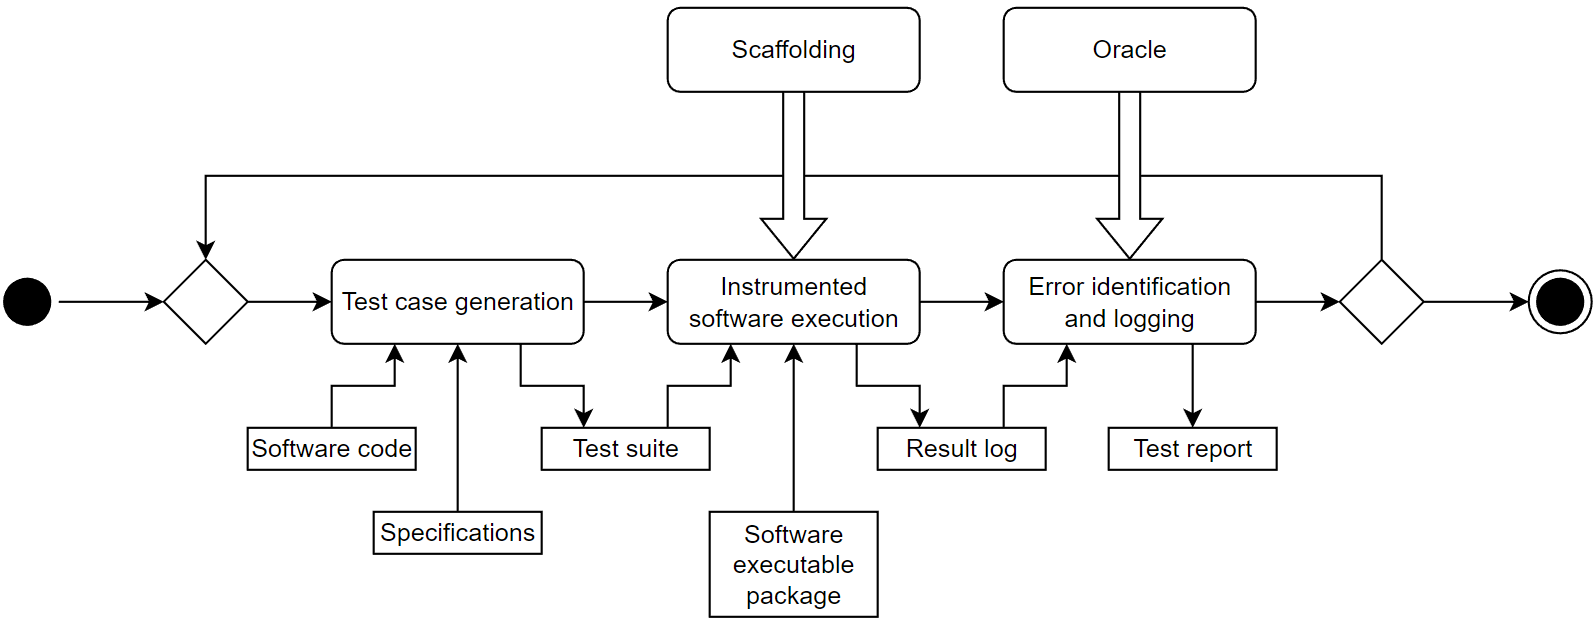
\includegraphics[width=0.75\linewidth]{images/twf.png}
    \caption{Testing workflow}
\end{figure}

\subsection{Test case generation}
We want to define good quality test sets. 
To do this we have to create artifacts that: 
\begin{itemize}
    \item Shows a high probability of finding errors. 
    \item Is able to cover an acceptable amount of cases. 
    \item Is sustainable (limited number of tests). 
\end{itemize}
Test cases can be defined manually. 
Test cases can be automatically generated (automated testing). 
The possible automated testing are: 
\begin{itemize}
    \item \textit{Combinatorial testing}: enumerate all possible inputs following some policy. 
    \item \textit{Concolic execution}: pseudo-random generation of inputs guided by symbolic path properties. 
    \item \textit{Fuzz testing (fuzzing)}: pseudo-random generation of inputs including invalid, unexpected inputs. 
    \item \textit{Search-based testing}: explores the space of valid inputs looking for those that improve some metrics. 
\end{itemize}

\paragraph*{Concrete symbolic execution}
The idea of concolic execution is to Perform symbolic execution alongside a concrete one (concrete inputs)
The state of concolic execution combine a symbolic part and a concrete part, used as needed to make progress in the exploration. 
The two steps followed by this technique are: 
\begin{enumerate}
    \item \textit{Concrete to symbolic}: derive conditions to explore new paths. 
    \item \textit{Symbolic to concrete}: simplify conditions to generate concrete inputs. 
\end{enumerate}
\begin{example}
    SLIDE 7
\end{example}
The advantages are: 
\begin{itemize}
    \item Can deal with black-box functions in path conditions (not possible with symbolic execution). 
    \item Can generate concrete test cases automatically, according to some code coverage criterion. 
\end{itemize} 
The limitations are: 
\begin{itemize}
    \item Faults typically occur with certain inputs only. 
        If faults are rare events, it's unlikely to spot them with concolic execution. 
    \item The number of paths explodes due to complex nested conditions that create large search space. 
    \item Does not guide the exploration, it just explores possible paths one by one as long as we have budget. 
\end{itemize}

<<<<<<< Updated upstream
\paragraph*{Fuzz testing}
=======




















>>>>>>> Stashed changes
